% Options for packages loaded elsewhere
% Options for packages loaded elsewhere
\PassOptionsToPackage{unicode}{hyperref}
\PassOptionsToPackage{hyphens}{url}
%
\documentclass[
  ignorenonframetext,
  aspectratio=169,
  russian,
]{beamer}
\newif\ifbibliography
\usepackage{pgfpages}
\setbeamertemplate{caption}[numbered]
\setbeamertemplate{caption label separator}{: }
\setbeamercolor{caption name}{fg=normal text.fg}
\beamertemplatenavigationsymbolshorizontal
% Prevent slide breaks in the middle of a paragraph
\widowpenalties 1 10000
\raggedbottom
\AtBeginPart{
  \frame{\partpage}
}
\AtBeginSection{
  \ifbibliography
  \else
    \frame{\sectionpage}
  \fi
}
\AtBeginSubsection{
  \frame{\subsectionpage}
}
\usepackage{iftex}
\ifPDFTeX
  \usepackage[T1]{fontenc}
  \usepackage[utf8]{inputenc}
  \usepackage{textcomp} % provide euro and other symbols
\else % if luatex or xetex
  \usepackage{unicode-math} % this also loads fontspec
  \defaultfontfeatures{Scale=MatchLowercase}
  \defaultfontfeatures[\rmfamily]{Ligatures=TeX,Scale=1}
\fi
\usepackage{lmodern}

\usetheme[]{metropolis}
\ifPDFTeX\else
  % xetex/luatex font selection
\fi
% Use upquote if available, for straight quotes in verbatim environments
\IfFileExists{upquote.sty}{\usepackage{upquote}}{}
\IfFileExists{microtype.sty}{% use microtype if available
  \usepackage[]{microtype}
  \UseMicrotypeSet[protrusion]{basicmath} % disable protrusion for tt fonts
}{}


\usepackage{longtable,booktabs,array}
\usepackage{calc} % for calculating minipage widths
\usepackage{caption}
% Make caption package work with longtable
\makeatletter
\def\fnum@table{\tablename~\thetable}
\makeatother
\usepackage{graphicx}
\makeatletter
\newsavebox\pandoc@box
\newcommand*\pandocbounded[1]{% scales image to fit in text height/width
  \sbox\pandoc@box{#1}%
  \Gscale@div\@tempa{\textheight}{\dimexpr\ht\pandoc@box+\dp\pandoc@box\relax}%
  \Gscale@div\@tempb{\linewidth}{\wd\pandoc@box}%
  \ifdim\@tempb\p@<\@tempa\p@\let\@tempa\@tempb\fi% select the smaller of both
  \ifdim\@tempa\p@<\p@\scalebox{\@tempa}{\usebox\pandoc@box}%
  \else\usebox{\pandoc@box}%
  \fi%
}
% Set default figure placement to htbp
\def\fps@figure{htbp}
\makeatother



\ifLuaTeX
\usepackage[bidi=basic,provide=*]{babel}
\else
\usepackage[bidi=default,provide=*]{babel}
\fi
% get rid of language-specific shorthands (see #6817):
\let\LanguageShortHands\languageshorthands
\def\languageshorthands#1{}


\setlength{\emergencystretch}{3em} % prevent overfull lines

\providecommand{\tightlist}{%
  \setlength{\itemsep}{0pt}\setlength{\parskip}{0pt}}



 

\usepackage[]{csquotes}

\IfFileExists{plex-otf.sty}{
  %% Full TeXlive
  % \usepackage[%
  %   % math,
  %   RM={Scale=0.94},SS={Scale=0.94},SScon={Scale=0.94},TT={Scale=MatchLowercase,FakeStretch=0.9},DefaultFeatures={Ligatures=Common}
  % ]{plex-otf}
}{
  %% TinyTeX
  \usepackage{libertine}
}

%%% Load theme
% https://deic.uab.cat/~iblanes/beamer_gallery/
\IfFileExists{beamerthemegotham.sty}{
  %% Full TeXlive
  \usetheme{gotham}
  \gothamset{
    numbering=totalpagenumber,
    parttocframe default=off,
    sectiontocframe default=off,
    subsectiontocframe default=off,
  }
}{
  %% TinyTeX
  \usetheme{Madrid}
}
\metroset{progressbar=frametitle,sectionpage=progressbar,numbering=fraction}
\makeatletter
\@ifpackageloaded{caption}{}{\usepackage{caption}}
\AtBeginDocument{%
\ifdefined\contentsname
  \renewcommand*\contentsname{Содержание}
\else
  \newcommand\contentsname{Содержание}
\fi
\ifdefined\listfigurename
  \renewcommand*\listfigurename{Список иллюстраций}
\else
  \newcommand\listfigurename{Список иллюстраций}
\fi
\ifdefined\listtablename
  \renewcommand*\listtablename{Список таблиц}
\else
  \newcommand\listtablename{Список таблиц}
\fi
\ifdefined\figurename
  \renewcommand*\figurename{Рисунок}
\else
  \newcommand\figurename{Рисунок}
\fi
\ifdefined\tablename
  \renewcommand*\tablename{Таблица}
\else
  \newcommand\tablename{Таблица}
\fi
}
\@ifpackageloaded{float}{}{\usepackage{float}}
\floatstyle{ruled}
\@ifundefined{c@chapter}{\newfloat{codelisting}{h}{lop}}{\newfloat{codelisting}{h}{lop}[chapter]}
\floatname{codelisting}{Список}
\newcommand*\listoflistings{\listof{codelisting}{Листинги}}
\makeatother
\makeatletter
\makeatother
\makeatletter
\@ifpackageloaded{caption}{}{\usepackage{caption}}
\@ifpackageloaded{subcaption}{}{\usepackage{subcaption}}
\makeatother

\usepackage{bookmark}
\IfFileExists{xurl.sty}{\usepackage{xurl}}{} % add URL line breaks if available
\urlstyle{same}
\hypersetup{
  pdftitle={Лабораторная работа №1},
  pdfauthor={Краснова К. Г., НКАбд-03-24},
  pdflang={ru-RU},
  hidelinks,
  pdfcreator={LaTeX via pandoc}}


\title{Лабораторная работа №1}
\subtitle{Основы информационной безопасности}
\author{Краснова К. Г., НКАбд-03-24}
\date{Invalid Date}
\institute{Российский университет дружбы народов, Москва, Россия}

\begin{document}
\frame{\titlepage}


\section{1. Информация}\label{ux438ux43dux444ux43eux440ux43cux430ux446ux438ux44f}

\begin{frame}{1.1 Докладчик}
\phantomsection\label{ux434ux43eux43aux43bux430ux434ux447ux438ux43a}
\begin{columns}[c]
\begin{column}{0.7\linewidth}
\begin{itemize}[<+->]
\tightlist
\item
  Кулябов Дмитрий Сергеевич
\item
  д.ф.-м.н., профессор
\item
  профессор кафедры теории вероятностей и кибербезопасности
\item
  Российский университет дружбы народов им. П. Лумумбы
\item
  \href{mailto:kulyabov-ds@rudn.ru}{\nolinkurl{kulyabov-ds@rudn.ru}}
\item
  \url{https://yamadharma.github.io/ru/}
\end{itemize}
\end{column}

\begin{column}{0.3\linewidth}
\pandocbounded{\includegraphics[keepaspectratio]{./image/kulyabov.jpg}}
\end{column}
\end{columns}
\end{frame}

\begin{frame}{1.2 Цель работы}
\phantomsection\label{ux446ux435ux43bux44c-ux440ux430ux431ux43eux442ux44b}
Получение практических навыков работы в консоли с атрибутами файлов,
закрепление теоретических основ дискреционного разграничения доступа в
современных системах с открытым кодом на базе ОС Linux
\end{frame}

\begin{frame}{1.3 Задание}
\phantomsection\label{ux437ux430ux434ux430ux43dux438ux435}
\begin{enumerate}[<+->]
\tightlist
\item
  Работа с атрибутами файлов
\item
  Заполнение таблицы \enquote{Установленные права и разрешённые
  действия} (см. табл. 2.1)
\item
  Заполнение таблицы \enquote{Минимальные права для совершения операций}
  (см. табл. 2.2)
\end{enumerate}
\end{frame}

\begin{frame}{1.4 Теоретическое введение}
\phantomsection\label{ux442ux435ux43eux440ux435ux442ux438ux447ux435ux441ux43aux43eux435-ux432ux432ux435ux434ux435ux43dux438ux435}
\textbf{Операционная система} --- это комплекс программ, предназначенных
для управления ресурсами компьютера и организации взаимодействия с
пользователем. {[}1{]}

\textbf{Права доступа} определяют, какие действия конкретный
пользователь может или не может совершать с определенным файлами и
каталогами. С помощью разрешений можно создать надежную среду --- такую,
в которой никто не может поменять содержимое ваших документов или
повредить системные файлы. {[}2{]}.
\end{frame}

\begin{frame}{1.5 Выполнение лабораторной работы}
\phantomsection\label{ux432ux44bux43fux43eux43bux43dux435ux43dux438ux435-ux43bux430ux431ux43eux440ux430ux442ux43eux440ux43dux43eux439-ux440ux430ux431ux43eux442ux44b}
Создаю нового пользователя quest через администратора
(рис.~\ref{fig-001}).

\begin{figure}

\centering{

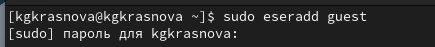
\includegraphics[width=0.7\linewidth,height=\textheight,keepaspectratio]{image/1.jpg}

}

\caption{\label{fig-001}Создание пользователя}

\end{figure}%
\end{frame}

\begin{frame}{1.6 Выполнение лабораторной работы}
\phantomsection\label{ux432ux44bux43fux43eux43bux43dux435ux43dux438ux435-ux43bux430ux431ux43eux440ux430ux442ux43eux440ux43dux43eux439-ux440ux430ux431ux43eux442ux44b-1}
Добавляю пароль для новой учетной записи (рис.~\ref{fig-002}).

\begin{figure}

\centering{

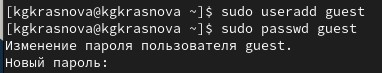
\includegraphics[width=0.7\linewidth,height=\textheight,keepaspectratio]{image/2.jpg}

}

\caption{\label{fig-002}Пароль1}

\end{figure}%
\end{frame}

\begin{frame}{1.7 Выполнение лабораторной работы}
\phantomsection\label{ux432ux44bux43fux43eux43bux43dux435ux43dux438ux435-ux43bux430ux431ux43eux440ux430ux442ux43eux440ux43dux43eux439-ux440ux430ux431ux43eux442ux44b-2}
Меняю пользователя на нового (рис.~\ref{fig-003}).

\begin{figure}

\centering{

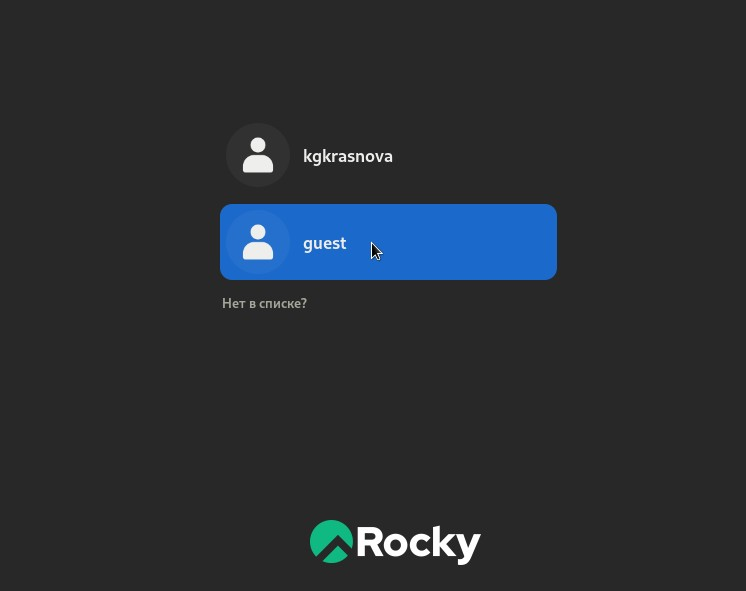
\includegraphics[width=0.7\linewidth,height=\textheight,keepaspectratio]{image/3.jpg}

}

\caption{\label{fig-003}Вход}

\end{figure}%
\end{frame}

\begin{frame}{1.8 Выполнение лабораторной работы}
\phantomsection\label{ux432ux44bux43fux43eux43bux43dux435ux43dux438ux435-ux43bux430ux431ux43eux440ux430ux442ux43eux440ux43dux43eux439-ux440ux430ux431ux43eux442ux44b-3}
Определяю, что нахожусь в нужной директории (рис.~\ref{fig-004}).

\begin{figure}

\centering{

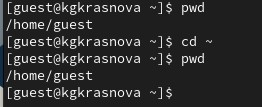
\includegraphics[width=0.7\linewidth,height=\textheight,keepaspectratio]{image/4.jpg}

}

\caption{\label{fig-004}pwd}

\end{figure}%
\end{frame}

\begin{frame}{1.9 Выполнение лабораторной работы}
\phantomsection\label{ux432ux44bux43fux43eux43bux43dux435ux43dux438ux435-ux43bux430ux431ux43eux440ux430ux442ux43eux440ux43dux43eux439-ux440ux430ux431ux43eux442ux44b-4}
Уточняю имя пользователя (рис.~\ref{fig-005}).

\begin{figure}

\centering{

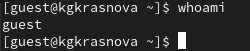
\includegraphics[width=0.7\linewidth,height=\textheight,keepaspectratio]{image/5.jpg}

}

\caption{\label{fig-005}имя пользователя}

\end{figure}%
\end{frame}

\begin{frame}{1.10 Выполнение лабораторной работы}
\phantomsection\label{ux432ux44bux43fux43eux43bux43dux435ux43dux438ux435-ux43bux430ux431ux43eux440ux430ux442ux43eux440ux43dux43eux439-ux440ux430ux431ux43eux442ux44b-5}
В выводе команды groups информация только о названии группы, к которой
относится пользователь. В выводе команды id можно найти больше
информации: имя пользователя и имя группы, также коды имени пользователя
и группы (рис.~\ref{fig-006}).

\begin{figure}

\centering{

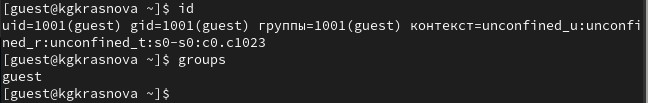
\includegraphics[width=0.7\linewidth,height=\textheight,keepaspectratio]{image/6.jpg}

}

\caption{\label{fig-006}Информация}

\end{figure}%
\end{frame}

\begin{frame}{1.11 Выполнение лабораторной работы}
\phantomsection\label{ux432ux44bux43fux43eux43bux43dux435ux43dux438ux435-ux43bux430ux431ux43eux440ux430ux442ux43eux440ux43dux43eux439-ux440ux430ux431ux43eux442ux44b-6}
Получаю информацию о пользователе с помощью команды
(рис.~\ref{fig-007}).

\begin{figure}

\centering{

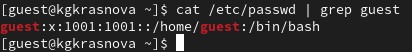
\includegraphics[width=0.7\linewidth,height=\textheight,keepaspectratio]{image/7.jpg}

}

\caption{\label{fig-007}Информация о пользователе}

\end{figure}%
\end{frame}

\begin{frame}{1.12 Выполнение лабораторной работы}
\phantomsection\label{ux432ux44bux43fux43eux43bux43dux435ux43dux438ux435-ux43bux430ux431ux43eux440ux430ux442ux43eux440ux43dux43eux439-ux440ux430ux431ux43eux442ux44b-7}
Да, список поддиректорий директории home получилось получить с помощью
команды ls -l, если мы добавим опцию -a, то сможем увидеть еще и
директорию пользователя root. Права у директории:

root: drwxr-xr-x(рис.~\ref{fig-008}).

\begin{figure}

\centering{

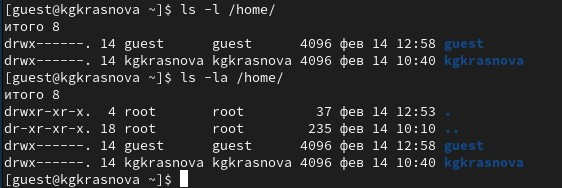
\includegraphics[width=0.7\linewidth,height=\textheight,keepaspectratio]{image/8.jpg}

}

\caption{\label{fig-008}Список}

\end{figure}%
\end{frame}

\begin{frame}{1.13 Выполнение лабораторной работы}
\phantomsection\label{ux432ux44bux43fux43eux43bux43dux435ux43dux438ux435-ux43bux430ux431ux43eux440ux430ux442ux43eux440ux43dux43eux439-ux440ux430ux431ux43eux442ux44b-8}
Пыталась проверить расширенные атрибуты директорий. Нет, их увидеть не
удалось (рис.~\ref{fig-009}).

\begin{figure}

\centering{

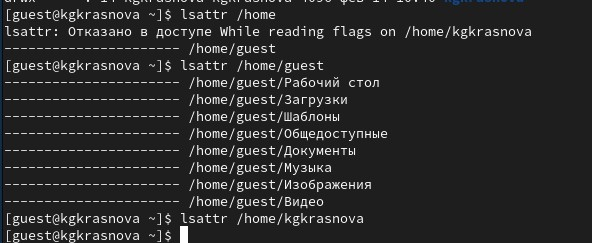
\includegraphics[width=0.7\linewidth,height=\textheight,keepaspectratio]{image/9.jpg}

}

\caption{\label{fig-009}Расширенные атрибуты}

\end{figure}%
\end{frame}

\begin{frame}{1.14 Выполнение лабораторной работы}
\phantomsection\label{ux432ux44bux43fux43eux43bux43dux435ux43dux438ux435-ux43bux430ux431ux43eux440ux430ux442ux43eux440ux43dux43eux439-ux440ux430ux431ux43eux442ux44b-9}
Создаю директорию. Расширенные атрибуты просмотреть не удается, но
атрибуты есть: drwxr-xr-x, их удалось просмотреть с помощью команды ls
-l (рис.~\ref{fig-010}).

\begin{figure}

\centering{

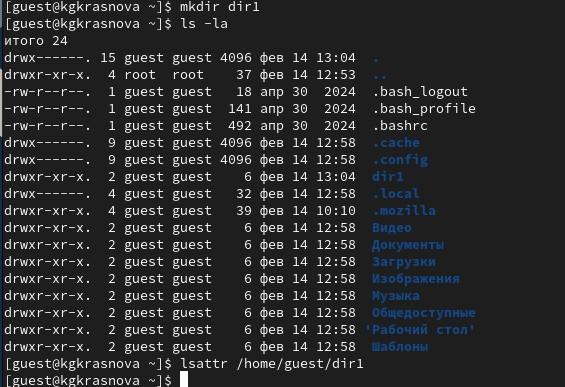
\includegraphics[width=0.7\linewidth,height=\textheight,keepaspectratio]{image/10.jpg}

}

\caption{\label{fig-010}Атрибуты директории}

\end{figure}%
\end{frame}

\begin{frame}{1.15 Выполнение лабораторной работы}
\phantomsection\label{ux432ux44bux43fux43eux43bux43dux435ux43dux438ux435-ux43bux430ux431ux43eux440ux430ux442ux43eux440ux43dux43eux439-ux440ux430ux431ux43eux442ux44b-10}
Снимаю атрибуты командой chmod 000 dir1, при проверке с помощью команды
ls -l видно, что теперь атрибуты действительно сняты
(рис.~\ref{fig-011}).

\begin{figure}

\centering{

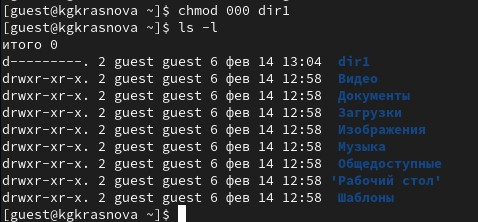
\includegraphics[width=0.7\linewidth,height=\textheight,keepaspectratio]{image/11.jpg}

}

\caption{\label{fig-011}Снятие атрибутов}

\end{figure}%
\end{frame}

\begin{frame}{1.16 Выполнение лабораторной работы}
\phantomsection\label{ux432ux44bux43fux43eux43bux43dux435ux43dux438ux435-ux43bux430ux431ux43eux440ux430ux442ux43eux440ux43dux43eux439-ux440ux430ux431ux43eux442ux44b-11}
Попытка создать файл в директории dir1. Выдает ошибку: \enquote{Отказано
в доступе} (рис.~\ref{fig-012}).

\begin{figure}

\centering{

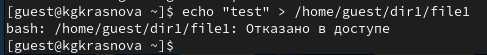
\includegraphics[width=0.7\linewidth,height=\textheight,keepaspectratio]{image/12.jpg}

}

\caption{\label{fig-012}Не удалось создать}

\end{figure}%
\end{frame}

\begin{frame}{1.17 Выполнение лабораторной работы}
\phantomsection\label{ux432ux44bux43fux43eux43bux43dux435ux43dux438ux435-ux43bux430ux431ux43eux440ux430ux442ux43eux440ux43dux43eux439-ux440ux430ux431ux43eux442ux44b-12}
Вернув права директории и использовав снова командy ls -l можно
убедиться, что файл не был создан (рис.~\ref{fig-013}).

\begin{figure}

\centering{

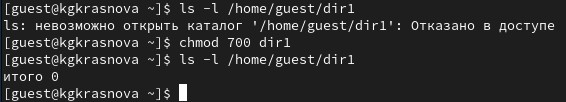
\includegraphics[width=0.7\linewidth,height=\textheight,keepaspectratio]{image/13.jpg}

}

\caption{\label{fig-013}Проверка}

\end{figure}%
\end{frame}

\begin{frame}{1.18 Заполнение таблицы 2.1}
\phantomsection\label{ux437ux430ux43fux43eux43bux43dux435ux43dux438ux435-ux442ux430ux431ux43bux438ux446ux44b-2.1}
\begin{longtable}[]{@{}
  >{\raggedright\arraybackslash}p{(\linewidth - 18\tabcolsep) * \real{0.1000}}
  >{\raggedright\arraybackslash}p{(\linewidth - 18\tabcolsep) * \real{0.1000}}
  >{\raggedright\arraybackslash}p{(\linewidth - 18\tabcolsep) * \real{0.1000}}
  >{\raggedright\arraybackslash}p{(\linewidth - 18\tabcolsep) * \real{0.1000}}
  >{\raggedright\arraybackslash}p{(\linewidth - 18\tabcolsep) * \real{0.1000}}
  >{\raggedright\arraybackslash}p{(\linewidth - 18\tabcolsep) * \real{0.1000}}
  >{\raggedright\arraybackslash}p{(\linewidth - 18\tabcolsep) * \real{0.1000}}
  >{\raggedright\arraybackslash}p{(\linewidth - 18\tabcolsep) * \real{0.1000}}
  >{\raggedright\arraybackslash}p{(\linewidth - 18\tabcolsep) * \real{0.1000}}
  >{\raggedright\arraybackslash}p{(\linewidth - 18\tabcolsep) * \real{0.1000}}@{}}
\toprule\noalign{}
\endhead
Права директории & Права файла & Создание файла & Удаление файла &
Запись в файл & Чтение файла & Смена директории & Просмотр файлов в
директории & Переимено- вание файла & Смена атрибутов файла \\
d(000) & (000) & - & - & - & - & - & - & - & - \\
d(000) & (100) & - & - & - & - & - & - & - & - \\
d(000) & (200) & - & - & - & - & - & - & - & - \\
d(000) & (300) & - & - & - & - & - & - & - & - \\
d(000) & (400) & - & - & - & - & - & - & - & - \\
d(000) & (500) & - & - & - & - & - & - & - & - \\
d(000) & (600) & - & - & - & - & - & - & - & - \\
d(000) & (700) & - & - & - & - & - & - & - & - \\
d(100) & (000) & - & - & - & - & + & - & - & + \\
d(100) & (100) & - & - & - & - & + & - & - & + \\
d(100) & (200) & - & - & + & - & + & - & - & + \\
d(100) & (300) & - & - & + & - & + & - & - & + \\
d(100) & (400) & - & - & - & + & + & - & - & + \\
d(100) & (500) & - & - & - & + & + & - & - & + \\
d(100) & (600) & - & - & + & + & + & - & - & + \\
d(100) & (700) & - & - & + & + & + & - & - & + \\
d(200) & (000) & - & - & - & - & - & - & - & - \\
d(200) & (100) & - & - & - & - & - & - & - & - \\
d(200) & (200) & - & - & - & - & - & - & - & - \\
d(200) & (300) & - & - & - & - & - & - & - & - \\
d(200) & (400) & - & - & - & - & - & - & - & - \\
d(200) & (500) & - & - & - & - & - & - & - & - \\
d(200) & (600) & - & - & - & - & - & - & - & - \\
d(200) & (700) & - & - & - & - & - & - & - & - \\
d(300) & (000) & + & + & - & - & + & - & + & + \\
d(300) & (100) & + & + & - & - & + & - & + & + \\
d(300) & (200) & + & + & + & - & + & - & + & + \\
d(300) & (300) & + & + & + & - & + & - & + & + \\
d(300) & (400) & + & + & - & + & + & - & + & + \\
d(300) & (500) & + & + & - & + & + & - & + & + \\
d(300) & (600) & + & + & + & + & + & - & + & + \\
d(300) & (700) & + & + & + & + & + & - & + & + \\
d(400) & (000) & - & - & - & - & - & + & - & - \\
d(400) & (100) & - & - & - & - & - & + & - & - \\
d(400) & (200) & - & - & - & - & - & + & - & - \\
d(400) & (300) & - & - & - & - & - & + & - & - \\
d(400) & (400) & - & - & - & - & - & + & - & - \\
d(400) & (500) & - & - & - & - & - & + & - & - \\
d(400) & (600) & - & - & - & - & - & + & - & - \\
d(400) & (700) & - & - & - & - & - & + & - & - \\
d(500) & (000) & - & - & - & - & + & + & - & + \\
d(500) & (100) & - & - & - & - & + & + & - & + \\
d(500) & (200) & - & - & + & - & + & + & - & + \\
d(500) & (300) & - & - & + & - & + & + & - & + \\
d(500) & (400) & - & - & - & + & + & + & - & + \\
d(500) & (500) & - & - & - & + & + & + & - & + \\
d(500) & (600) & - & - & + & + & + & + & - & + \\
d(500) & (700) & - & - & + & + & + & + & - & + \\
d(600) & (000) & - & - & - & - & - & + & - & - \\
d(600) & (100) & - & - & - & - & - & + & - & - \\
d(600) & (200) & - & - & - & - & - & + & - & - \\
d(600) & (300) & - & - & - & - & - & + & - & - \\
d(600) & (400) & - & - & - & - & - & + & - & - \\
d(600) & (500) & - & - & - & - & - & + & - & - \\
d(600) & (600) & - & - & - & - & - & + & - & - \\
d(600) & (700) & - & - & - & - & - & + & - & - \\
d(700) & (000) & + & + & - & - & + & + & + & + \\
d(700) & (100) & + & + & - & - & + & + & + & + \\
d(700) & (200) & + & + & + & - & + & + & + & + \\
d(700) & (300) & + & + & + & - & + & + & + & + \\
d(700) & (400) & + & + & - & + & + & + & + & + \\
d(700) & (500) & + & + & - & + & + & + & + & + \\
d(700) & (600) & + & + & + & + & + & + & + & + \\
d(700) & (700) & + & + & + & + & + & + & + & + \\
\bottomrule\noalign{}
\end{longtable}

Таблица 2.1 «Установленные права и разрешённые действия»
\end{frame}

\begin{frame}{1.19 Выполнение лабораторной работы}
\phantomsection\label{ux432ux44bux43fux43eux43bux43dux435ux43dux438ux435-ux43bux430ux431ux43eux440ux430ux442ux43eux440ux43dux43eux439-ux440ux430ux431ux43eux442ux44b-13}
Пример заполнения таблицы 2.1 (рис.~\ref{fig-014}).

\begin{figure}

\centering{

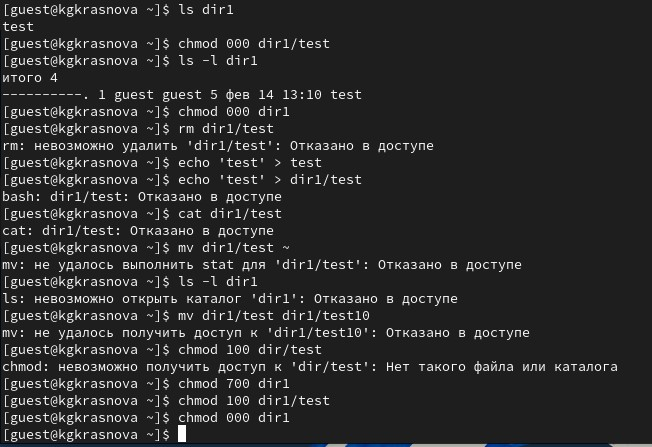
\includegraphics[width=0.7\linewidth,height=\textheight,keepaspectratio]{image/14.jpg}

}

\caption{\label{fig-014}Таблица 2.1}

\end{figure}%
\end{frame}

\begin{frame}{1.20 Заполнение таблицы 2.2}
\phantomsection\label{ux437ux430ux43fux43eux43bux43dux435ux43dux438ux435-ux442ux430ux431ux43bux438ux446ux44b-2.2}
\begin{longtable}[]{@{}
  >{\raggedright\arraybackslash}p{(\linewidth - 8\tabcolsep) * \real{0.2000}}
  >{\raggedright\arraybackslash}p{(\linewidth - 8\tabcolsep) * \real{0.2000}}
  >{\raggedright\arraybackslash}p{(\linewidth - 8\tabcolsep) * \real{0.2000}}
  >{\raggedright\arraybackslash}p{(\linewidth - 8\tabcolsep) * \real{0.2000}}
  >{\raggedright\arraybackslash}p{(\linewidth - 8\tabcolsep) * \real{0.2000}}@{}}
\toprule\noalign{}
\endhead
Операция & & Минимальные права на директорию & & Минимальные права на
файл \\
Создание файла & & d(300) & & - \\
Удаление файла & & d(300) & & - \\
Чтение файла & & d(100) & & (400) \\
Запись в файл & & d(100) & & (200) \\
Переименование файла & & d(300) & & (000) \\
Создание поддиректории & & d(300) & & - \\
Удаление поддиректории & & d(300) & & - \\
\bottomrule\noalign{}
\end{longtable}

Таблица 2.2 \enquote{Минимальные права для совершения операций}
\end{frame}

\begin{frame}{1.21 Выполнение лабораторной работы}
\phantomsection\label{ux432ux44bux43fux43eux43bux43dux435ux43dux438ux435-ux43bux430ux431ux43eux440ux430ux442ux43eux440ux43dux43eux439-ux440ux430ux431ux43eux442ux44b-14}
Пример заполнения таблицы 2.2 (рис.~\ref{fig-015}).

\begin{figure}

\centering{

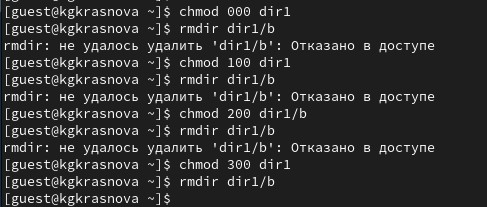
\includegraphics[width=0.7\linewidth,height=\textheight,keepaspectratio]{image/15.jpg}

}

\caption{\label{fig-015}Таблица 2.2}

\end{figure}%
\end{frame}

\begin{frame}{1.22 Выводы}
\phantomsection\label{ux432ux44bux432ux43eux434ux44b}
Были получены практические навыки работы в консоли с атрибутами файлов,
закреплены теоретические основы дискреционного разграничения доступа в
современных системах с открытым кодом на базе ОС Linux.
\end{frame}




\end{document}
